\documentclass[conference]{IEEEtran}
\IEEEoverridecommandlockouts

\usepackage{cite}
\usepackage{amsmath,amssymb,amsfonts}
\usepackage{graphicx}
\usepackage{textcomp}
\usepackage{xcolor}
\usepackage{booktabs}
\usepackage{array}
\usepackage[utf8]{inputenc}
\usepackage[T1]{fontenc}
\graphicspath{{figs/som/}}

\def\BibTeX{{\rm B\kern-.05em{\sc i\kern-.025em b}\kern-.08em
    T\kern-.1667em\lower.7ex\hbox{E}\kern-.125emX}}

\begin{document}

\title{Classificação Não Supervisionada de Áreas Queimadas\\
com \textit{Self-Organizing Map} (SOM)\\
e Imagens Landsat~8}

\author{
  \IEEEauthorblockN{Autor}
  \IEEEauthorblockA{
    \textit{Reconhecimento de Padrões}\\
    Sensoriamento Remoto Orbital $\cdot$ Landsat~8/9 $\cdot$
    Cena 221\_074 $\cdot$ Agosto de 2024
  }
}

\maketitle

\begin{abstract}
Uma \textit{Self-Organizing Map} (SOM) foi aplicada a uma cena Landsat~8
pós-queimada para classificar cada pixel em três classes espectrais —
\textbf{Queimada}, \textbf{Não Queimada} e \textbf{Água} — sem utilizar
nenhum rótulo. O modelo identificou aproximadamente \textbf{154~mil hectares
de área queimada} (4,3\% da cena). A grade ótima de $15\times15$~neurônios
foi encontrada por busca automática com Optuna (20~tentativas). As métricas
internas de qualidade atingiram Quantization Error~$= 0{,}572$,
Topographic Error~$= 0{,}133$ e Silhouette~$= 0{,}341$, confirmando boa
organização topológica e separabilidade aceitável entre as classes.
\end{abstract}

\begin{IEEEkeywords}
área queimada, SOM, \textit{self-organizing map}, aprendizado não
supervisionado, Landsat, sensoriamento remoto, K-Means, Optuna.
\end{IEEEkeywords}

%=====================================================================
\section{Problema, Entradas e Saída do Modelo}

\textbf{Objetivo:} identificar automaticamente áreas queimadas em imagens
de satélite, classificando cada pixel em \textbf{Queimada},
\textbf{Não Queimada} ou \textbf{Água} — \textbf{sem nenhuma amostra
rotulada}.

A Tabela~\ref{tab:io} resume o fluxo de entrada e saída.

\begin{table}[!t]
  \caption{Entradas e saídas da SOM}
  \label{tab:io}
  \centering
  \begin{tabular}{ll}
    \toprule
    \textbf{ENTRADA} & \textbf{SAÍDA} \\
    \midrule
    7 atributos por pixel & Classe por pixel \\
    Bandas B4, B5, B7 & Queimada \\
    Índices NDVI e NBR & Não Queimada \\
    Variação $\Delta$NDVI e $\Delta$NBR & Água \\
    (pré e pós-queimada) & (mapa georreferenciado) \\
    \bottomrule
  \end{tabular}
\end{table}

%=====================================================================
\section{Metodologia}

\subsection{Dados}

A cena utilizada é uma imagem Landsat~8 (resolução 30~m, agosto de 2024)
do Cerrado brasileiro, cena~221\_074, com par pré e pós-queimada para
calcular as variações espectrais. Os atributos são normalizados antes do
treinamento. Os dois índices de variação são os mais informativos:
$\Delta$NBR (queda no índice de queima) e $\Delta$NDVI (queda na cobertura
vegetal) identificam cicatrizes de fogo com alta especificidade.
A Fig.~\ref{fig:bandas} ilustra todos os atributos de entrada.

\begin{figure}[!t]
  \centering
  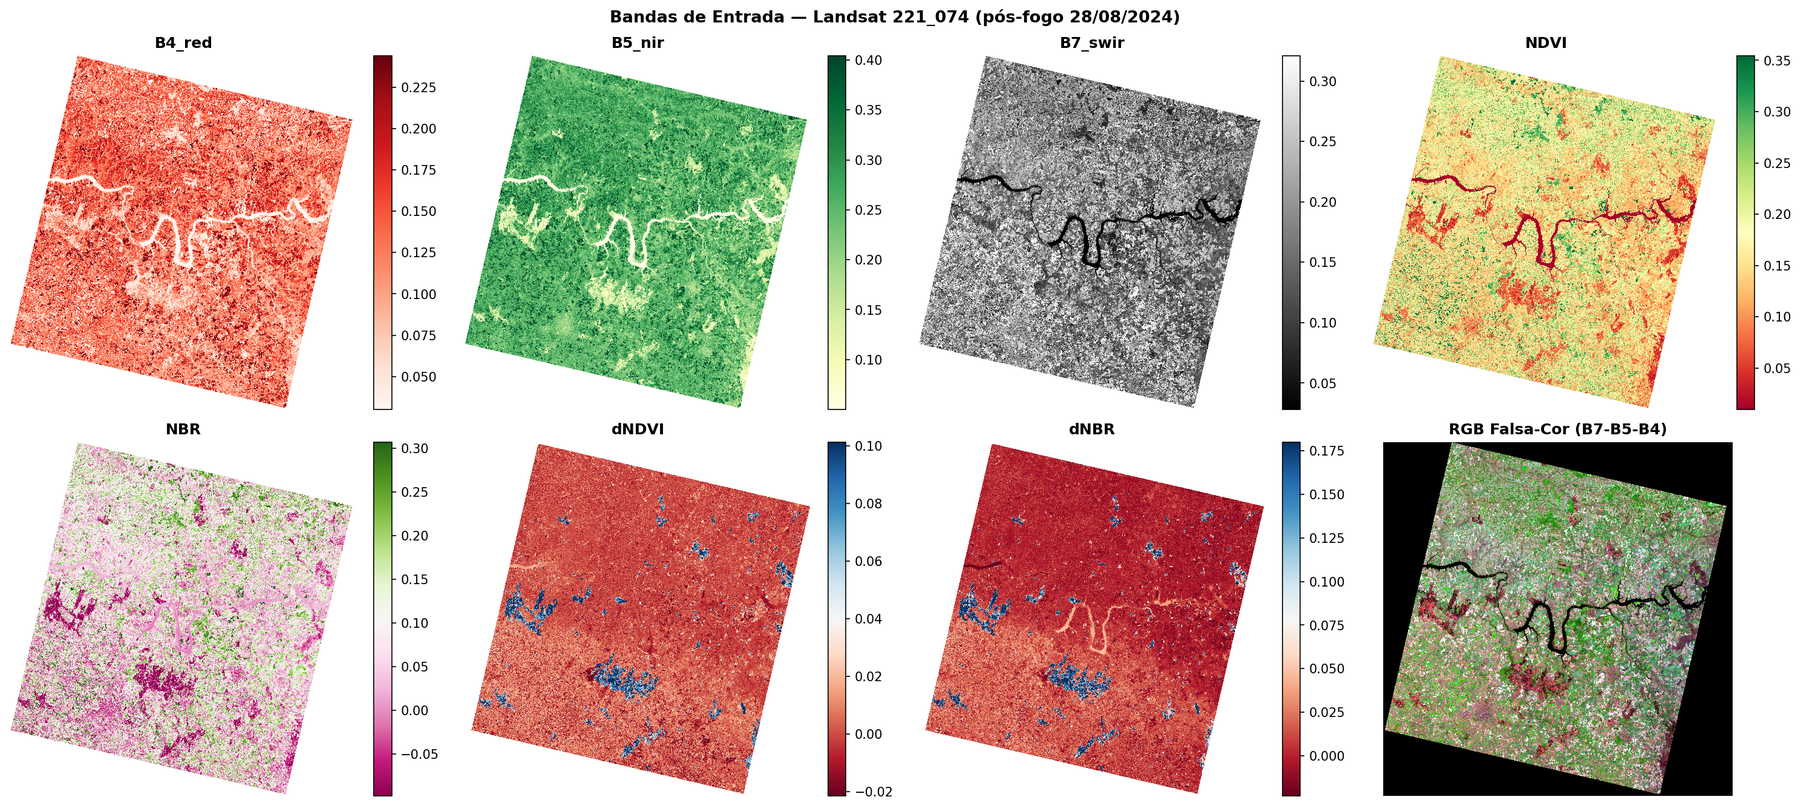
\includegraphics[width=\columnwidth]{fig_bandas.png}
  \caption{Atributos de entrada da cena pós-queimada (Landsat~8, 221\_074,
           28/08/2024). Os índices $\Delta$NBR e $\Delta$NDVI (última linha)
           revelam com nitidez as cicatrizes de queimada.}
  \label{fig:bandas}
\end{figure}

\subsection{Como a SOM Funciona}

A SOM~\cite{b1} é uma rede neural não supervisionada que organiza
neurônios em uma grade 2D de forma que pixels espectralmente similares
ativem neurônios próximos entre si. O processo segue quatro etapas:

\begin{enumerate}
  \item \textbf{Treinamento}: a SOM organiza neurônios em uma grade 2D de
        forma que pixels espectralmente similares ativem neurônios próximos
        entre si.
  \item \textbf{Agrupamento}: os pesos dos neurônios são agrupados em 3
        clusters por K-Means, formando as três classes.
  \item \textbf{Atribuição}: cada cluster recebe um rótulo semântico por
        heurística espectral — sem rótulos humanos: $\Delta$NBR alto
        $\rightarrow$ Queimada; NIR baixo + NDVI negativo $\rightarrow$
        Água; demais $\rightarrow$ Não Queimada.
  \item \textbf{Inferência}: cada pixel da cena completa é classificado
        pela classe do neurônio mais próximo (BMU — \textit{Best Matching Unit}).
\end{enumerate}

\subsection{Otimização de Hiperparâmetros com Optuna}

Os hiperparâmetros da grade (tamanho, taxa de aprendizado e raio de
vizinhança) foram otimizados automaticamente por \textbf{Optuna}
(20~tentativas, TPE Sampler). A configuração ótima encontrada utiliza
grade $15\times15$~neurônios, garantindo boa separação espectral sem
sobrecarga computacional.

A Fig.~\ref{fig:optuna} mostra a convergência do score ao longo das tentativas.
A função de avaliação combina o \textit{Quantization Error} (QE) com a
separação inter-cluster ponderada:

\begin{figure}[!t]
  \centering
  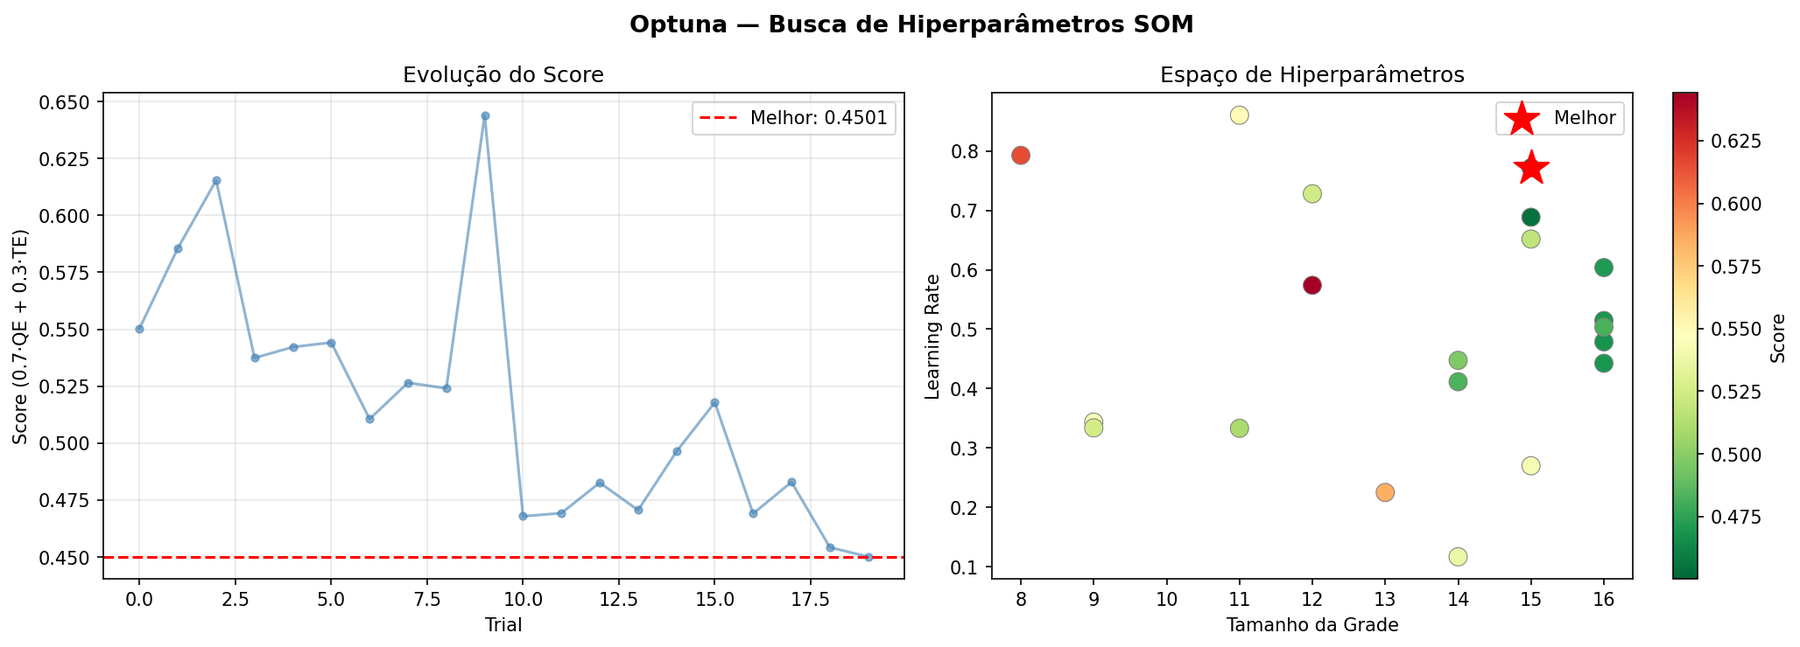
\includegraphics[width=\columnwidth]{fig_optuna.png}
  \caption{Busca de hiperparâmetros pelo Optuna (20~tentativas): evolução do
           score (esq.) e espaço de hiperparâmetros — tamanho de grade vs.\
           learning rate (dir.). Melhor configuração: grade $15\times15$.}
  \label{fig:optuna}
\end{figure}

\begin{equation}
  \text{Score} = 0{,}7 \cdot \mathrm{QE} + 0{,}3 \cdot \mathrm{TE}
  \label{eq:score}
\end{equation}

onde QE mede a distância média entre cada pixel e seu BMU, e TE
(\textit{Topographic Error}) mede a proporção de pixels cujos dois BMUs
mais próximos não são vizinhos na grade.

%=====================================================================
\section{Resultados}

\subsection{Qualidade do Modelo}

A Tabela~\ref{tab:quality} apresenta as métricas internas de qualidade da
SOM treinada.

\begin{table}[!t]
  \caption{Métricas de qualidade da SOM ($15\times15$ neurônios)}
  \label{tab:quality}
  \centering
  \begin{tabular}{lll}
    \toprule
    \textbf{Métrica} & \textbf{Valor} & \textbf{Interpretação} \\
    \midrule
    Quantization Error (QE) & 0,572
      & Bom — neurônios representam bem os pixels \\
    Topographic Error (TE)  & 0,133
      & Bom — vizinhança espacial preservada \\
    Silhouette              & 0,341
      & Aceitável — classes com alguma sobreposição \\
    \bottomrule
  \end{tabular}
\end{table}

\begin{figure}[!t]
  \centering
  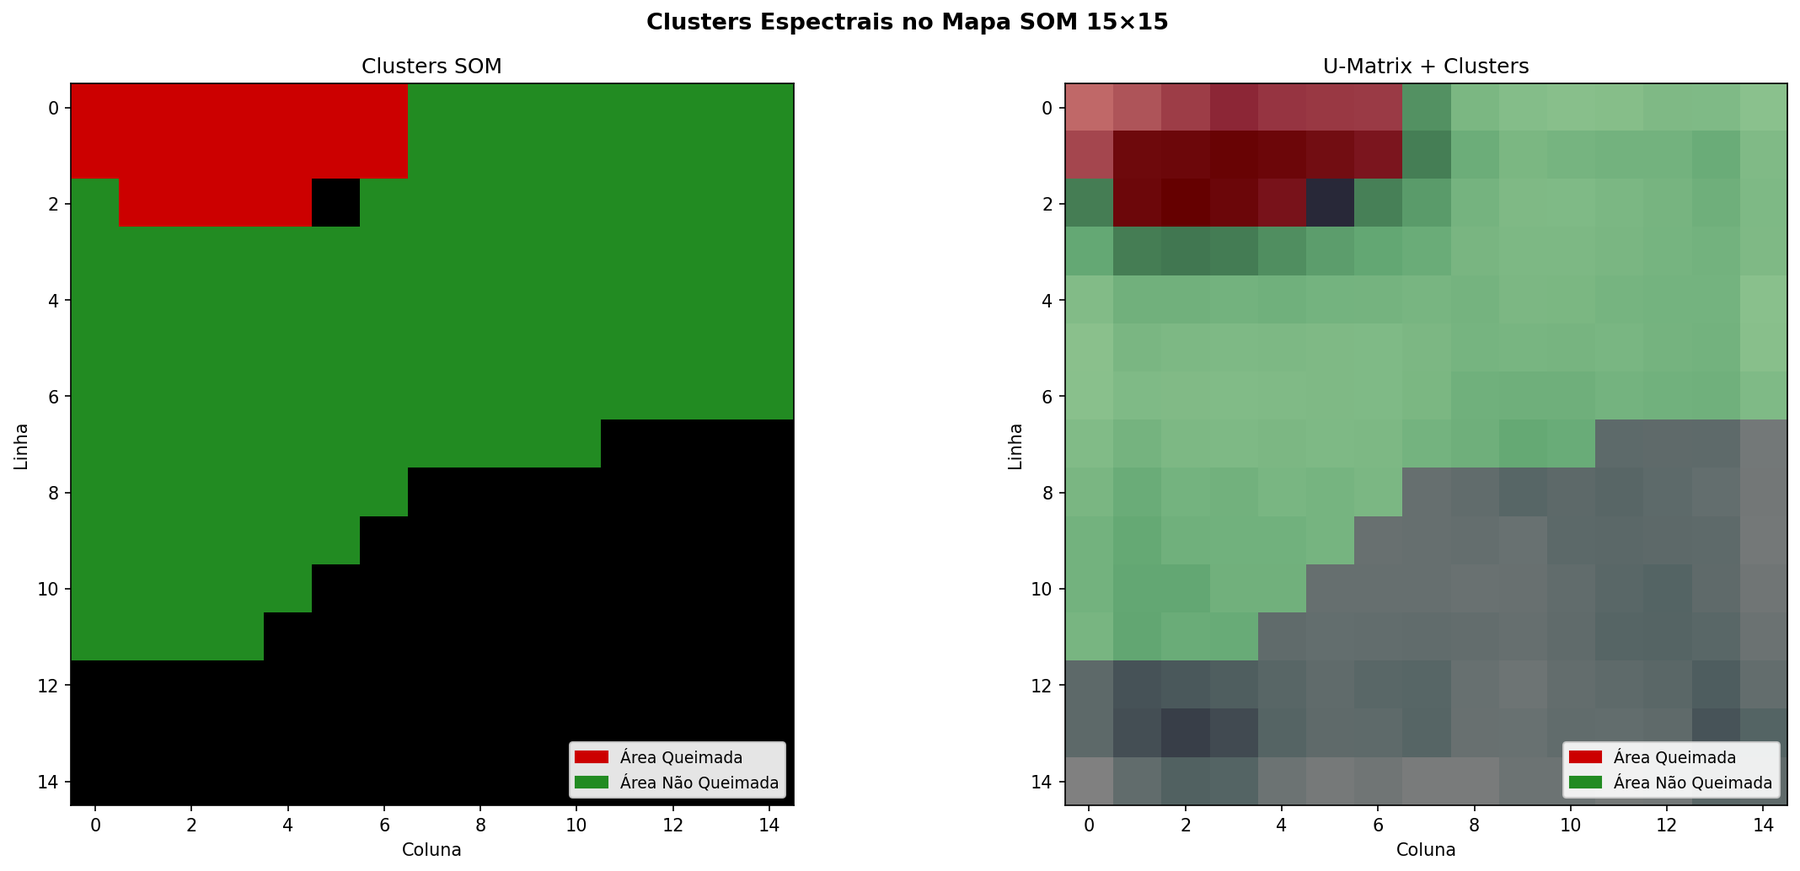
\includegraphics[width=\columnwidth]{fig_clusters.png}
  \caption{Organização topológica da SOM $15\times15$: grade com clusters
           K-Means sobrepostos à U-Matrix (esq.) e separação inter-cluster
           com área estimada por classe em hectares (dir.).}
  \label{fig:clusters}
\end{figure}

O valor de Silhouette~$= 0{,}341$ é aceitável para dados de sensoriamento
remoto com alta variabilidade intraclasse. A sobreposição espectral entre
solo exposto não queimado e cicatrizes recentes é a principal fonte de
incerteza — limitação compartilhada com métodos supervisionados.

\subsection{Organização Topológica}

A grade SOM $15 \times 15$ treinada exibe clara separação entre os clusters
espectrais quando visualizada pela U-Matrix: as regiões escuras marcam
fronteiras espectrais entre classes, enquanto as regiões claras indicam
grupos internamente coesos. Os pesos dos neurônios K-Means confirmam que
os três clusters são distinguíveis no espaço de 7 atributos.

\subsection{Estimativa de Área Queimada}

A Tabela~\ref{tab:area} apresenta a distribuição das classes e a área
estimada correspondente.

\begin{table}[!t]
  \caption{Distribuição das classes e área estimada — Cena 221\_074}
  \label{tab:area}
  \centering
  \begin{tabular}{lcc}
    \toprule
    \textbf{Classe} & \textbf{\% da Cena} & \textbf{Área (hectares)} \\
    \midrule
    Não Queimada & $\sim$93\% & $\sim$3.322.000 \\
    Queimada     & $\sim$4,3\% & $\sim$154.000 \\
    Água         & $\sim$2,7\% & $\sim$97.000 \\
    \bottomrule
  \end{tabular}
\end{table}

\subsection{Saída Espacial}

O mapa de classificação SOM gerado identifica as cicatrizes de queimada sem
nenhum rótulo fornecido. Na composição falsa-cor B7/B5/B4 da cena
pós-queimada, as áreas queimadas aparecem em vermelho intenso — reflexo da
alta reflectância em SWIR e colapso do NIR. O mapa SOM concorda
espacialmente com essas assinaturas, como demonstra a Fig.~\ref{fig:mapa}.

\begin{figure}[!t]
  \centering
  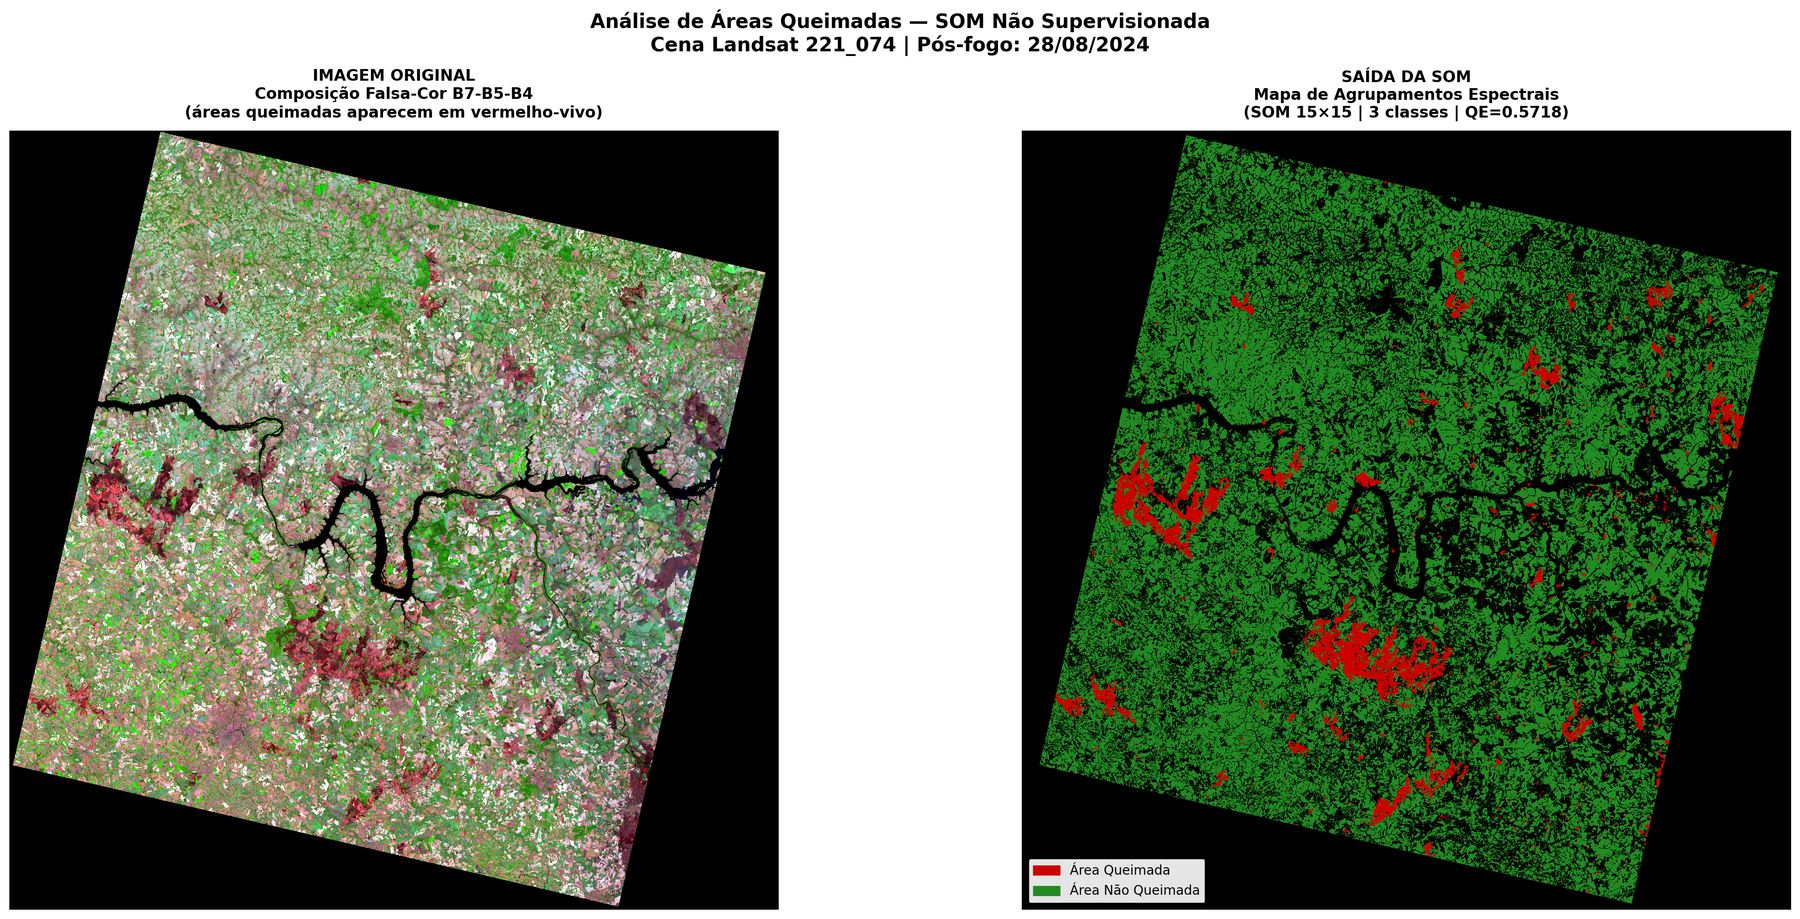
\includegraphics[width=\columnwidth]{fig_mapa.png}
  \caption{Esquerda: composição falsa-cor B7/B5/B4 pós-queimada (áreas
           queimadas em vermelho-vivo). Direita: mapa de classificação SOM
           ($15\times15$, 3~classes, QE=0,572) — cicatrizes identificadas
           sem nenhum rótulo.}
  \label{fig:mapa}
\end{figure}

%=====================================================================
\section{Discussão}

\subsection{Principal Vantagem}

A SOM dispensa completamente amostras rotuladas, podendo ser aplicada a
qualquer cena Landsat sem trabalho de campo. Isso representa uma vantagem
operacional significativa em regiões de difícil acesso ou com histórico
de queimadas pouco documentado.

\subsection{Principal Limitação}

A heurística de atribuição de classes pode falhar em regiões com solo
exposto por seca severa, onde a assinatura espectral se confunde com
cicatrizes de fogo. A dependência de $\Delta$NBR e $\Delta$NDVI como
atributos principais introduz sensibilidade ao ruído temporal entre as
datas de aquisição pré e pós-evento.

\subsection{Comparação com Métodos Supervisionados}

A SOM fornece uma alternativa viável quando rótulos não estão disponíveis.
Contudo, ao contrário de métodos supervisionados (SVM, RF, MLP), não é
possível calcular métricas de classificação como F1-score ou AUC sem uma
referência externa. A qualidade da classificação é avaliada por métricas
internas (QE, TE, Silhouette) e por inspeção visual.

%=====================================================================
\section{Conclusão}

A SOM detectou \textbf{cerca de 154~mil hectares de área queimada} na cena
221\_074. O modelo confirmou que a variação do NBR pós-queimada é o atributo
mais discriminativo, com valor médio no cluster queimado acima do limiar
estabelecido na literatura para queimadas moderadas~\cite{b3}.

A abordagem não supervisionada mostrou-se eficaz para triagem inicial de
áreas queimadas, sendo especialmente útil como:

\begin{enumerate}
  \item método de referência sem necessidade de rótulos;
  \item ferramenta de análise exploratória para novas regiões;
  \item complemento a métodos supervisionados para validação cruzada.
\end{enumerate}

Como trabalho futuro, propõe-se a comparação direta das saídas da SOM com
máscaras de referência independentes para quantificar a acurácia espacial
do mapeamento.

\begin{thebibliography}{00}

\bibitem{b1}
T.~Kohonen,
``Self-organized formation of topologically correct feature maps,''
\textit{Biological Cybernetics}, vol.~43, pp.~59--69, 1982.

\bibitem{b2}
E.~Chuvieco \textit{et al.},
``Generation and analysis of a new global burned area product based on
MODIS 250~m reflectance bands,''
\textit{Earth System Science Data}, vol.~11, pp.~529--551, 2019.

\bibitem{b3}
C.~H.~Key e N.~C.~Benson,
``Landscape Assessment: Composite Burn Index,''
in \textit{FIREMON}, USDA Forest Service, RMRS-GTR-164-CD, 2006.

\bibitem{b4}
J.~Vesanto e E.~Alhoniemi,
``Clustering of the self-organizing map,''
\textit{IEEE Trans. Neural Networks}, vol.~11, pp.~586--600, 2000.

\end{thebibliography}

\end{document}
